\problemname{Stacks of Books}

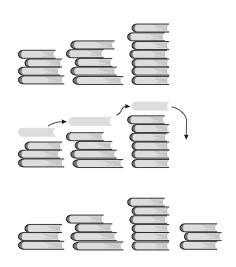
\includegraphics{Travar.png}

On a table there are a number of stacks of books. Each day, one book is taken from each stack. These books together form a new stack to the right of the others, see figure 1. If a stack becomes empty, the stacks are pushed together from the right. Since there is a finite number of books, sooner or later the same arrangement will recur. Your task is to write a program that asks for the initial arrangement and then determines how long it takes before a previously seen arrangement recurs.

\begin{tabular}{|c|c|c|c|c|c|c|}
\hline
Day&Stack 1&Stack 2&Stack 3&Stack 4&Stack 5&Stack 6\\\hline
1&4&5&7&&&\\
2&3&4&6&3&&\\
3&2&3&5&2&4&\\
4&1&2&4&1&3&5\\
5&1&3&2&4&6&\\
6&2&1&3&5&5&\\
7&\textbf{1}&\textbf{2}&\textbf{4}&\textbf{4}&\textbf{5}&\\
8&1&3&3&4&5&\\
9&2&2&3&4&5&\\
10&1&1&2&3&4&5\\
11&1&2&3&4&6&\\
12&1&2&3&5&5&\\
13&\textbf{1}&\textbf{2}&\textbf{4}&\textbf{4}&\textbf{5}&\\\hline
\end{tabular}

The table above shows how the number of books in the stacks varies over 13 days. In the upcoming tests, the number of books is $\le 50$, the number of stacks is at most $\le 15$, and the number of days is $\le 100$.

\section*{Input}
The first line consists of an integer --- the number of book stacks $N$.
The next line consists of $N$ integers --- the number of books in the stacks.

\section*{Output}
The output should consist of two integers --- the two first days where the arrangement was repeated. The first day should be output first.
